\chapter{Graph Adjacency Lists and Matrices}

\setcounter{problem}{1}
\section{Discussion}

\begin{fullwidth}

The goal of this task is to teach you about the implementation of graphs in Python and how to implement a few simple related algorithms.  As part of this exercise, you will also learn to transform data, which is an important data preparation skill you will need as an analyst.   In this project, you will convert a string that looks like this:

\begin{alltt}\small
parrt: tombu, dmose, parrt
tombu: dmose, kg9s
dmose: tombu
kg9s: dmose
\end{alltt}

\noindent to an adjacency list representation and ultimately generate a visual representation via \href{http://www.graphviz.org/}{\textcolor{blue}{graphviz/dot}}:

\begin{center}
\scalebox{.55}{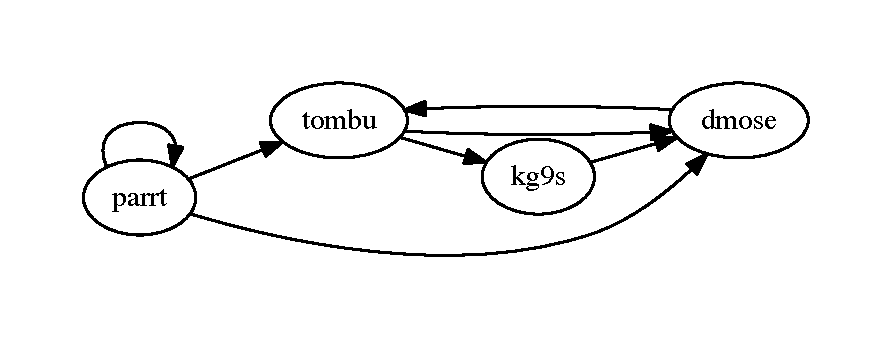
\includegraphics{figures/email-graph.pdf}}
\end{center}

\noindent For fun, you will also create an edge matrix representation:

\[
\bordermatrix{
~ & parrt & tombu & dmose & kg9s \cr
parrt & 1 & 1 & 1 & 0\cr
tombu & 0 & 0 & 1 & 1 \cr
dmose & 0 & 1 & 0 & 0 \cr
kg9s & 0 & 0 & 1 & 0\cr
}
\]

\noindent where the nodes have the following indexes:
 
\[
\left[
\begin{array}{c}
1: parrt \\
2: tombu \\
3: dmose \\
4: kg9s \\
\end{array}
\right]
\]

The following sections describe the functions you must create in {\tt graph.py}. See a starter kit I've built for you and placed in canvas as file {\tt graph\_starterkit.py}, but of course you will rename it to {\tt graph.py}.

\subsection{Processing an adjacency list string}

First, you have to process a string representation of an adjacency list and create an internal data structure:

\begin{pyverbatim}
def adjlist(adj_list):
    """
    Read in adj list and store in form of dict mapping node
    name to list of outgoing edges. Preserve the order you find
    for the nodes.
    """
    ...
\end{pyverbatim}

You will use an ordered dictionary ({\tt OrderedDict}) that maps node name x to a list of target nodes. x will be a string and the target list will be a list of strings. For example, from line in string adj\_list

\begin{alltt}
parrt: tombu, dmose, parrt
\end{alltt}

\noindent you will create an entry in the dictionary with key {\tt parrt} and value:

\begin{pyverbatim}
['tombu', 'dmose', 'parrt']
\end{pyverbatim}

\noindent To process the text, you must split the incoming string into lines and then process them one at a time as each line represents an adjacency list. You will use string functions {\tt split} and (likely) {\tt strip} to process the text.

\noindent Printing the adjacency list dictionary from {\tt adjlist}, I see:

\begin{pyverbatim}
OrderedDict([('parrt', ['tombu', 'dmose', 'parrt']),
 ('tombu', ['dmose', 'kg9s']), 
 ('dmose', ['tombu']), 
 ('kg9s', ['dmose'])])
\end{pyverbatim}

\subsection{Adjacency list to adjacency matrix}

Given an adjacency list stored as a dictionary, create a function that converts that to an adjacency matrix:
 
\begin{pyverbatim}
def adjmatrix(adj):
    """
    From an adjacency list, return the adjacency matrix with entries in {0,1}.
    The order of nodes in adj is assumed to be same as they were read in.
    """
    ...
\end{pyverbatim}

\noindent The matrix should look like the one shown above.

\subsection{Getting a list of all nodes}

A very useful function to have is the following that returns a list of all nodes visited starting at a particular node in a graph. 
 
\begin{pyverbatim}
def nodes(adj, start_node):
    """
    Walk every node in graph described by adj list starting at start_node
    using a breadth-first search.  Return a list of all nodes found (in
    any order). Include the start_node.
    """
    ...
\end{pyverbatim}

\noindent Do not build a recursive function as you must do a breadth-first search. (Recursive functions are much more useful when doing a depth-first search.) The basic algorithm looks like this:

\begin{algorithm}[H]
\SetInd{.3em}{.3em}
add the start node to a work list\;
\While{more work}{
    node = remove a node from work list\;
    add node to node list\;
    add node to visited list\;
    targets = adjacency\_list[node]\;
    add all unvisited targets to work list\;
}
\Return{nodes}\;
\end{algorithm}

\subsection{Generating DOT output}

In order to visualize the graph you have read in, create the following function that dumps valid Graphviz DOT code. Then cut-and-paste the output and put it into Graphviz to display it.
 
\begin{pyverbatim}
def gendot(adj):
    """
    Return a string representing the graph in Graphviz DOT format
    with all p->q edges.
    """
    ...
\end{pyverbatim}

\noindent For the adjacency list shown at the start of this assignment, you should to generate the following DOT code:

\begin{alltt}\small
digraph g \{
  rankdir=LR;
  parrt -> tombu;
  parrt -> dmose;
  parrt -> parrt;
  tombu -> dmose;
  tombu -> kg9s;
  dmose -> tombu;
  kg9s -> dmose;
\}
\end{alltt}

\section{Testing}

I have provided a {\tt test\_graph.py} test rig via canvas that exercises the required functions using the adjacency list described here. Please make sure that your library works with this test rig.

\section{Deliverables}

Please submit the following via canvas:
 
\begin{itemize}
\item {\tt graphs.py}
\item a text file with the output of running {\tt test\_graph.py}
\item a PDF showing the visual representation of the graph as generated by graphviz/dot
\end{itemize}

\end{fullwidth}
